
%%%%%

Using instead the geometric mean makes the order of aggregation and
scaling immaterial since the ratio of geometric means is the same as
the geometric mean of ratios.  Figure \ref{fig:geometric-mean} shows how the
results in forecasting would change if one replaces the arithmetic mean by the
geometric mean. 

%%%%%

We also investigate the effect of lengthening the time window to include 2021. 
\begin{itemize}
\item For forecasting: results get better, whether we look at
  non-adjusted (first plot) or adjusted scores (second plot).  Other
  than that, interpretation is qualitatively similar, except fb now
  seems to be worse than gs.  And \chngcli~is strong, even in the
  non-adjusted view.
  \item For hotspots: Alden will write something explaining why we
    don't do hotspot detection in 2021.
\end{itemize}


%%%%% 

We look at various approaches to
accounting for the fact that the \gs~indicator is only available
for XX HRRs.

\begin{itemize}
  \item For forecasting task: clearly gs is not missing at random, and when it's present, it tends to be predictive.  Hence high values have a low false positivity rate.  Most visible in the adjusted view below, where gs triumphs.  Also \chngcli~gets a lot worse.

\item For hotspots: All methods look better, suggesting that the “GS locations” are easier for hotspot prediction. E.g. at 7-days ahead, the AUCs computed based on all locations range from 0.61-0.66; restricted to GS locations, the AUCs range from about 0.65-0.69. (These are all eyeballed, should get actual numbers if we want to say something like this in paper.)
\item gs\_subset appears to be particularly helped by this subsetting
  (which makes sense since on those other locations it was 0-imputed)
  \item Daniel will also try gs\_impute as in forecasting
\end{itemize}

%%%%%

Figure \ref{fig:finalized-vs-honest} quantifies the effect of
not properly accounting for the question of ``what was known when'' in
performing retrospective evaluations of forecasters.  When methods are
given the finalized version of the data rather than the version available at the time that the forecast would have been made, all methods
appear (falsely) to have better performance.  For example, for forecasting case rates
7-days ahead, the WIS of all methods is at least 8\% larger than what would have been
recorded using the finalized values of the data.  This effect
diminishes as the forecasting horizon increases, reflecting the fact
that these forecasters rely less heavily on recent data than very
short-term forecasters.  Crucially, some methods are
``helped'' more than others by the less scrupulous retrospective
evaluation, underscoring the difficulty of avoiding misleading
conclusions when performing retrospective evaluations of forecasters.

The \chngcli~indicator (along with the other claims-based signals) is the most
affected by this distinction, reflecting the latency in claims-based
reporting. \attn{Actually, \dv~is the least affected for forecasting
  whereas it is one of the most affected for hotspots.}  This supports
the importance of efforts to provide ``nowcasts'' for claims signals
(which corresponds to a 0-ahead ``forecast'' of what the claims
signal's value will be once all data has been collected).

Even the \ar~model is affected by this distinction, reflecting the
fact that the case rates themselves (i.e., the response values) are also
subject to revision.  The forecasters based on indicators are thus
affected both by revisions to the indicators and by revisions to the
case rates.

\begin{itemize}
%\item Motivates the importance of nowcasting for claims signals.
  \item For forecasting task: Also, \chngcli~and \dv~perform very similarly here, which is
    reassuring because they're measuring the same thing (in
    principle).  Yet they must have very different backfill profiles…
  \item For hotspots task: dv seems to get a bigger boost than
    \chngcov - interesting dichotomy to forecasting
\item But in both forecasting/hotspots \chngcli~is affected a lot by backfill
\item \attn{We should be careful about which indicators we were not
      able to track latency for.  In fact, we should probably remove
      these from the plot since they would be more strongly affected
      than is shown in the plot.}

\item \attn{We can also discuss the distinction
      between indicators that could in principle have low latency
      (e.g. GS) versus those where latency is inherent
      (e.g. claims-based indicators). If the goal is assessing the
      performance of GS ``for the next pandemic'' then it would make
      sense to give GS a pass since in theory they could have had it
      with very low latency (as opposed to claims based signals where
      backfill may be unavoidable).  Of course, in
    ``the next pandemic'' there might not be such highly specific
    symptoms such as A+A as there was in the COVID-19 case.} 
\end{itemize}

\begin{figure}[t]
     \centering
     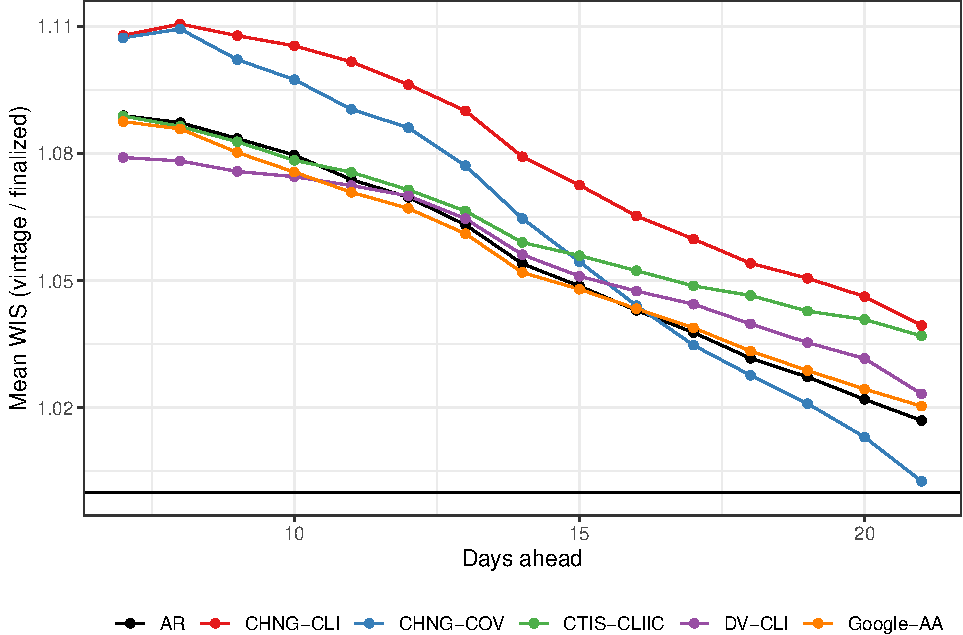
\includegraphics[width=\textwidth]{fig/fcast-honest-v-finalized-1.pdf}
     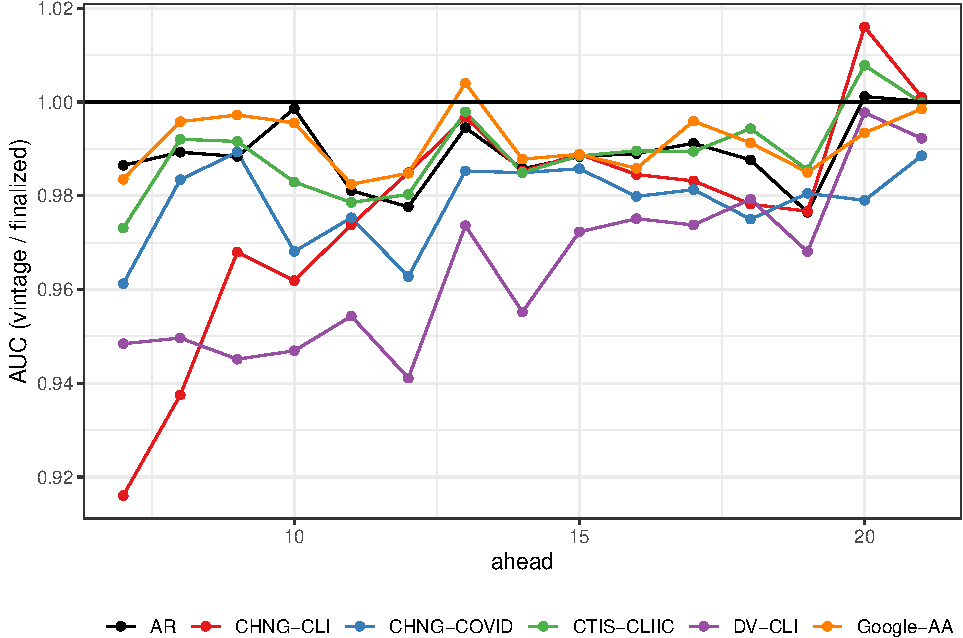
\includegraphics[width=\textwidth]{fig/hot-honest-v-finalized-1.pdf}
     \caption{How misleading is a retrospective analysis that uses the
       finalized version of the data rather than the version that was
       in fact available at the time the forecast was made?  Plots
       show the ratio in performance (using mean WIS fore the
       forecasting task and AUC for the hotspot prediction
       task). \label{fig:finalized-vs-honest} Cheating vs. honest plots.} 
\end{figure}

